\documentclass[noauthor,handout]{ximera}
%handout:  for handout version with no solutions or instructor notes
%handout,instructornotes:  for instructor version with just problems and notes, no solutions
%noinstructornotes:  shows only problem and solutions

%% handout
%% space
%% newpage
%% numbers
%% nooutcomes

%I added the commands here so that I would't have to keep looking them up
%\newcommand{\RR}{\mathbb R}
%\renewcommand{\d}{\,d}
%\newcommand{\dd}[2][]{\frac{d #1}{d #2}}
%\renewcommand{\l}{\ell}
%\newcommand{\ddx}{\frac{d}{dx}}
%\everymath{\displaystyle}
%\newcommand{\dfn}{\textbf}
%\newcommand{\eval}[1]{\bigg[ #1 \bigg]}

%\begin{image}
%\includegraphics[trim= 170 420 250 180]{Figure1.pdf}
%\end{image}

%add a ``.'' below when used in a specific directory.

%%\usepackage{todonotes}
%\usepackage{mathtools} %% Required for wide table Curl and Greens
%\usepackage{cuted} %% Required for wide table Curl and Greens
\newcommand{\todo}{}

\usepackage{esint} % for \oiint
\ifxake%%https://math.meta.stackexchange.com/questions/9973/how-do-you-render-a-closed-surface-double-integral
\renewcommand{\oiint}{{\large\bigcirc}\kern-1.56em\iint}
\fi


\graphicspath{
  {./}
  {ximeraTutorial/}
  {basicPhilosophy/}
  {functionsOfSeveralVariables/}
  {normalVectors/}
  {lagrangeMultipliers/}
  {vectorFields/}
  {greensTheorem/}
  {shapeOfThingsToCome/}
  {dotProducts/}
  {partialDerivativesAndTheGradientVector/}
  {../productAndQuotientRules/exercises/}
  {../normalVectors/exercisesParametricPlots/}
  {../continuityOfFunctionsOfSeveralVariables/exercises/}
  {../partialDerivativesAndTheGradientVector/exercises/}
  {../directionalDerivativeAndChainRule/exercises/}
  {../commonCoordinates/exercisesCylindricalCoordinates/}
  {../commonCoordinates/exercisesSphericalCoordinates/}
  {../greensTheorem/exercisesCurlAndLineIntegrals/}
  {../greensTheorem/exercisesDivergenceAndLineIntegrals/}
  {../shapeOfThingsToCome/exercisesDivergenceTheorem/}
  {../greensTheorem/}
  {../shapeOfThingsToCome/}
  {../separableDifferentialEquations/exercises/}
  {vectorFields/}
}

\newcommand{\mooculus}{\textsf{\textbf{MOOC}\textnormal{\textsf{ULUS}}}}

\usepackage{tkz-euclide}\usepackage{tikz}
\usepackage{tikz-cd}
\usetikzlibrary{arrows}
\tikzset{>=stealth,commutative diagrams/.cd,
  arrow style=tikz,diagrams={>=stealth}} %% cool arrow head
\tikzset{shorten <>/.style={ shorten >=#1, shorten <=#1 } } %% allows shorter vectors

\usetikzlibrary{backgrounds} %% for boxes around graphs
\usetikzlibrary{shapes,positioning}  %% Clouds and stars
\usetikzlibrary{matrix} %% for matrix
\usepgfplotslibrary{polar} %% for polar plots
\usepgfplotslibrary{fillbetween} %% to shade area between curves in TikZ
\usetkzobj{all}
\usepackage[makeroom]{cancel} %% for strike outs
%\usepackage{mathtools} %% for pretty underbrace % Breaks Ximera
%\usepackage{multicol}
\usepackage{pgffor} %% required for integral for loops



%% http://tex.stackexchange.com/questions/66490/drawing-a-tikz-arc-specifying-the-center
%% Draws beach ball
\tikzset{pics/carc/.style args={#1:#2:#3}{code={\draw[pic actions] (#1:#3) arc(#1:#2:#3);}}}



\usepackage{array}
\setlength{\extrarowheight}{+.1cm}
\newdimen\digitwidth
\settowidth\digitwidth{9}
\def\divrule#1#2{
\noalign{\moveright#1\digitwidth
\vbox{\hrule width#2\digitwidth}}}





\newcommand{\RR}{\mathbb R}
\newcommand{\R}{\mathbb R}
\newcommand{\N}{\mathbb N}
\newcommand{\Z}{\mathbb Z}

\newcommand{\sagemath}{\textsf{SageMath}}


%\renewcommand{\d}{\,d\!}
\renewcommand{\d}{\mathop{}\!d}
\newcommand{\dd}[2][]{\frac{\d #1}{\d #2}}
\newcommand{\pp}[2][]{\frac{\partial #1}{\partial #2}}
\renewcommand{\l}{\ell}
\newcommand{\ddx}{\frac{d}{\d x}}

\newcommand{\zeroOverZero}{\ensuremath{\boldsymbol{\tfrac{0}{0}}}}
\newcommand{\inftyOverInfty}{\ensuremath{\boldsymbol{\tfrac{\infty}{\infty}}}}
\newcommand{\zeroOverInfty}{\ensuremath{\boldsymbol{\tfrac{0}{\infty}}}}
\newcommand{\zeroTimesInfty}{\ensuremath{\small\boldsymbol{0\cdot \infty}}}
\newcommand{\inftyMinusInfty}{\ensuremath{\small\boldsymbol{\infty - \infty}}}
\newcommand{\oneToInfty}{\ensuremath{\boldsymbol{1^\infty}}}
\newcommand{\zeroToZero}{\ensuremath{\boldsymbol{0^0}}}
\newcommand{\inftyToZero}{\ensuremath{\boldsymbol{\infty^0}}}



\newcommand{\numOverZero}{\ensuremath{\boldsymbol{\tfrac{\#}{0}}}}
\newcommand{\dfn}{\textbf}
%\newcommand{\unit}{\,\mathrm}
\newcommand{\unit}{\mathop{}\!\mathrm}
\newcommand{\eval}[1]{\bigg[ #1 \bigg]}
\newcommand{\seq}[1]{\left( #1 \right)}
\renewcommand{\epsilon}{\varepsilon}
\renewcommand{\phi}{\varphi}


\renewcommand{\iff}{\Leftrightarrow}

\DeclareMathOperator{\arccot}{arccot}
\DeclareMathOperator{\arcsec}{arcsec}
\DeclareMathOperator{\arccsc}{arccsc}
\DeclareMathOperator{\si}{Si}
\DeclareMathOperator{\scal}{scal}
\DeclareMathOperator{\sign}{sign}


%% \newcommand{\tightoverset}[2]{% for arrow vec
%%   \mathop{#2}\limits^{\vbox to -.5ex{\kern-0.75ex\hbox{$#1$}\vss}}}
\newcommand{\arrowvec}[1]{{\overset{\rightharpoonup}{#1}}}
%\renewcommand{\vec}[1]{\arrowvec{\mathbf{#1}}}
\renewcommand{\vec}[1]{{\overset{\boldsymbol{\rightharpoonup}}{\mathbf{#1}}}\hspace{0in}}

\newcommand{\point}[1]{\left(#1\right)} %this allows \vector{ to be changed to \vector{ with a quick find and replace
\newcommand{\pt}[1]{\mathbf{#1}} %this allows \vec{ to be changed to \vec{ with a quick find and replace
\newcommand{\Lim}[2]{\lim_{\point{#1} \to \point{#2}}} %Bart, I changed this to point since I want to use it.  It runs through both of the exercise and exerciseE files in limits section, which is why it was in each document to start with.

\DeclareMathOperator{\proj}{\mathbf{proj}}
\newcommand{\veci}{{\boldsymbol{\hat{\imath}}}}
\newcommand{\vecj}{{\boldsymbol{\hat{\jmath}}}}
\newcommand{\veck}{{\boldsymbol{\hat{k}}}}
\newcommand{\vecl}{\vec{\boldsymbol{\l}}}
\newcommand{\uvec}[1]{\mathbf{\hat{#1}}}
\newcommand{\utan}{\mathbf{\hat{t}}}
\newcommand{\unormal}{\mathbf{\hat{n}}}
\newcommand{\ubinormal}{\mathbf{\hat{b}}}

\newcommand{\dotp}{\bullet}
\newcommand{\cross}{\boldsymbol\times}
\newcommand{\grad}{\boldsymbol\nabla}
\newcommand{\divergence}{\grad\dotp}
\newcommand{\curl}{\grad\cross}
%\DeclareMathOperator{\divergence}{divergence}
%\DeclareMathOperator{\curl}[1]{\grad\cross #1}
\newcommand{\lto}{\mathop{\longrightarrow\,}\limits}

\renewcommand{\bar}{\overline}

\colorlet{textColor}{black}
\colorlet{background}{white}
\colorlet{penColor}{blue!50!black} % Color of a curve in a plot
\colorlet{penColor2}{red!50!black}% Color of a curve in a plot
\colorlet{penColor3}{red!50!blue} % Color of a curve in a plot
\colorlet{penColor4}{green!50!black} % Color of a curve in a plot
\colorlet{penColor5}{orange!80!black} % Color of a curve in a plot
\colorlet{penColor6}{yellow!70!black} % Color of a curve in a plot
\colorlet{fill1}{penColor!20} % Color of fill in a plot
\colorlet{fill2}{penColor2!20} % Color of fill in a plot
\colorlet{fillp}{fill1} % Color of positive area
\colorlet{filln}{penColor2!20} % Color of negative area
\colorlet{fill3}{penColor3!20} % Fill
\colorlet{fill4}{penColor4!20} % Fill
\colorlet{fill5}{penColor5!20} % Fill
\colorlet{gridColor}{gray!50} % Color of grid in a plot

\newcommand{\surfaceColor}{violet}
\newcommand{\surfaceColorTwo}{redyellow}
\newcommand{\sliceColor}{greenyellow}




\pgfmathdeclarefunction{gauss}{2}{% gives gaussian
  \pgfmathparse{1/(#2*sqrt(2*pi))*exp(-((x-#1)^2)/(2*#2^2))}%
}


%%%%%%%%%%%%%
%% Vectors
%%%%%%%%%%%%%

%% Simple horiz vectors
\renewcommand{\vector}[1]{\left\langle #1\right\rangle}


%% %% Complex Horiz Vectors with angle brackets
%% \makeatletter
%% \renewcommand{\vector}[2][ , ]{\left\langle%
%%   \def\nextitem{\def\nextitem{#1}}%
%%   \@for \el:=#2\do{\nextitem\el}\right\rangle%
%% }
%% \makeatother

%% %% Vertical Vectors
%% \def\vector#1{\begin{bmatrix}\vecListA#1,,\end{bmatrix}}
%% \def\vecListA#1,{\if,#1,\else #1\cr \expandafter \vecListA \fi}

%%%%%%%%%%%%%
%% End of vectors
%%%%%%%%%%%%%

%\newcommand{\fullwidth}{}
%\newcommand{\normalwidth}{}



%% makes a snazzy t-chart for evaluating functions
%\newenvironment{tchart}{\rowcolors{2}{}{background!90!textColor}\array}{\endarray}

%%This is to help with formatting on future title pages.
\newenvironment{sectionOutcomes}{}{}



%% Flowchart stuff
%\tikzstyle{startstop} = [rectangle, rounded corners, minimum width=3cm, minimum height=1cm,text centered, draw=black]
%\tikzstyle{question} = [rectangle, minimum width=3cm, minimum height=1cm, text centered, draw=black]
%\tikzstyle{decision} = [trapezium, trapezium left angle=70, trapezium right angle=110, minimum width=3cm, minimum height=1cm, text centered, draw=black]
%\tikzstyle{question} = [rectangle, rounded corners, minimum width=3cm, minimum height=1cm,text centered, draw=black]
%\tikzstyle{process} = [rectangle, minimum width=3cm, minimum height=1cm, text centered, draw=black]
%\tikzstyle{decision} = [trapezium, trapezium left angle=70, trapezium right angle=110, minimum width=3cm, minimum height=1cm, text centered, draw=black]

%\usepackage{todonotes}
%\usepackage{mathtools} %% Required for wide table Curl and Greens
%\usepackage{cuted} %% Required for wide table Curl and Greens
\newcommand{\todo}{}

\usepackage{esint} % for \oiint
\ifxake%%https://math.meta.stackexchange.com/questions/9973/how-do-you-render-a-closed-surface-double-integral
\renewcommand{\oiint}{{\large\bigcirc}\kern-1.56em\iint}
\fi


\graphicspath{
  {./}
  {ximeraTutorial/}
  {basicPhilosophy/}
  {functionsOfSeveralVariables/}
  {normalVectors/}
  {lagrangeMultipliers/}
  {vectorFields/}
  {greensTheorem/}
  {shapeOfThingsToCome/}
  {dotProducts/}
  {partialDerivativesAndTheGradientVector/}
  {../productAndQuotientRules/exercises/}
  {../normalVectors/exercisesParametricPlots/}
  {../continuityOfFunctionsOfSeveralVariables/exercises/}
  {../partialDerivativesAndTheGradientVector/exercises/}
  {../directionalDerivativeAndChainRule/exercises/}
  {../commonCoordinates/exercisesCylindricalCoordinates/}
  {../commonCoordinates/exercisesSphericalCoordinates/}
  {../greensTheorem/exercisesCurlAndLineIntegrals/}
  {../greensTheorem/exercisesDivergenceAndLineIntegrals/}
  {../shapeOfThingsToCome/exercisesDivergenceTheorem/}
  {../greensTheorem/}
  {../shapeOfThingsToCome/}
  {../separableDifferentialEquations/exercises/}
  {vectorFields/}
}

\newcommand{\mooculus}{\textsf{\textbf{MOOC}\textnormal{\textsf{ULUS}}}}

\usepackage{tkz-euclide}\usepackage{tikz}
\usepackage{tikz-cd}
\usetikzlibrary{arrows}
\tikzset{>=stealth,commutative diagrams/.cd,
  arrow style=tikz,diagrams={>=stealth}} %% cool arrow head
\tikzset{shorten <>/.style={ shorten >=#1, shorten <=#1 } } %% allows shorter vectors

\usetikzlibrary{backgrounds} %% for boxes around graphs
\usetikzlibrary{shapes,positioning}  %% Clouds and stars
\usetikzlibrary{matrix} %% for matrix
\usepgfplotslibrary{polar} %% for polar plots
\usepgfplotslibrary{fillbetween} %% to shade area between curves in TikZ
\usetkzobj{all}
\usepackage[makeroom]{cancel} %% for strike outs
%\usepackage{mathtools} %% for pretty underbrace % Breaks Ximera
%\usepackage{multicol}
\usepackage{pgffor} %% required for integral for loops



%% http://tex.stackexchange.com/questions/66490/drawing-a-tikz-arc-specifying-the-center
%% Draws beach ball
\tikzset{pics/carc/.style args={#1:#2:#3}{code={\draw[pic actions] (#1:#3) arc(#1:#2:#3);}}}



\usepackage{array}
\setlength{\extrarowheight}{+.1cm}
\newdimen\digitwidth
\settowidth\digitwidth{9}
\def\divrule#1#2{
\noalign{\moveright#1\digitwidth
\vbox{\hrule width#2\digitwidth}}}





\newcommand{\RR}{\mathbb R}
\newcommand{\R}{\mathbb R}
\newcommand{\N}{\mathbb N}
\newcommand{\Z}{\mathbb Z}

\newcommand{\sagemath}{\textsf{SageMath}}


%\renewcommand{\d}{\,d\!}
\renewcommand{\d}{\mathop{}\!d}
\newcommand{\dd}[2][]{\frac{\d #1}{\d #2}}
\newcommand{\pp}[2][]{\frac{\partial #1}{\partial #2}}
\renewcommand{\l}{\ell}
\newcommand{\ddx}{\frac{d}{\d x}}

\newcommand{\zeroOverZero}{\ensuremath{\boldsymbol{\tfrac{0}{0}}}}
\newcommand{\inftyOverInfty}{\ensuremath{\boldsymbol{\tfrac{\infty}{\infty}}}}
\newcommand{\zeroOverInfty}{\ensuremath{\boldsymbol{\tfrac{0}{\infty}}}}
\newcommand{\zeroTimesInfty}{\ensuremath{\small\boldsymbol{0\cdot \infty}}}
\newcommand{\inftyMinusInfty}{\ensuremath{\small\boldsymbol{\infty - \infty}}}
\newcommand{\oneToInfty}{\ensuremath{\boldsymbol{1^\infty}}}
\newcommand{\zeroToZero}{\ensuremath{\boldsymbol{0^0}}}
\newcommand{\inftyToZero}{\ensuremath{\boldsymbol{\infty^0}}}



\newcommand{\numOverZero}{\ensuremath{\boldsymbol{\tfrac{\#}{0}}}}
\newcommand{\dfn}{\textbf}
%\newcommand{\unit}{\,\mathrm}
\newcommand{\unit}{\mathop{}\!\mathrm}
\newcommand{\eval}[1]{\bigg[ #1 \bigg]}
\newcommand{\seq}[1]{\left( #1 \right)}
\renewcommand{\epsilon}{\varepsilon}
\renewcommand{\phi}{\varphi}


\renewcommand{\iff}{\Leftrightarrow}

\DeclareMathOperator{\arccot}{arccot}
\DeclareMathOperator{\arcsec}{arcsec}
\DeclareMathOperator{\arccsc}{arccsc}
\DeclareMathOperator{\si}{Si}
\DeclareMathOperator{\scal}{scal}
\DeclareMathOperator{\sign}{sign}


%% \newcommand{\tightoverset}[2]{% for arrow vec
%%   \mathop{#2}\limits^{\vbox to -.5ex{\kern-0.75ex\hbox{$#1$}\vss}}}
\newcommand{\arrowvec}[1]{{\overset{\rightharpoonup}{#1}}}
%\renewcommand{\vec}[1]{\arrowvec{\mathbf{#1}}}
\renewcommand{\vec}[1]{{\overset{\boldsymbol{\rightharpoonup}}{\mathbf{#1}}}\hspace{0in}}

\newcommand{\point}[1]{\left(#1\right)} %this allows \vector{ to be changed to \vector{ with a quick find and replace
\newcommand{\pt}[1]{\mathbf{#1}} %this allows \vec{ to be changed to \vec{ with a quick find and replace
\newcommand{\Lim}[2]{\lim_{\point{#1} \to \point{#2}}} %Bart, I changed this to point since I want to use it.  It runs through both of the exercise and exerciseE files in limits section, which is why it was in each document to start with.

\DeclareMathOperator{\proj}{\mathbf{proj}}
\newcommand{\veci}{{\boldsymbol{\hat{\imath}}}}
\newcommand{\vecj}{{\boldsymbol{\hat{\jmath}}}}
\newcommand{\veck}{{\boldsymbol{\hat{k}}}}
\newcommand{\vecl}{\vec{\boldsymbol{\l}}}
\newcommand{\uvec}[1]{\mathbf{\hat{#1}}}
\newcommand{\utan}{\mathbf{\hat{t}}}
\newcommand{\unormal}{\mathbf{\hat{n}}}
\newcommand{\ubinormal}{\mathbf{\hat{b}}}

\newcommand{\dotp}{\bullet}
\newcommand{\cross}{\boldsymbol\times}
\newcommand{\grad}{\boldsymbol\nabla}
\newcommand{\divergence}{\grad\dotp}
\newcommand{\curl}{\grad\cross}
%\DeclareMathOperator{\divergence}{divergence}
%\DeclareMathOperator{\curl}[1]{\grad\cross #1}
\newcommand{\lto}{\mathop{\longrightarrow\,}\limits}

\renewcommand{\bar}{\overline}

\colorlet{textColor}{black}
\colorlet{background}{white}
\colorlet{penColor}{blue!50!black} % Color of a curve in a plot
\colorlet{penColor2}{red!50!black}% Color of a curve in a plot
\colorlet{penColor3}{red!50!blue} % Color of a curve in a plot
\colorlet{penColor4}{green!50!black} % Color of a curve in a plot
\colorlet{penColor5}{orange!80!black} % Color of a curve in a plot
\colorlet{penColor6}{yellow!70!black} % Color of a curve in a plot
\colorlet{fill1}{penColor!20} % Color of fill in a plot
\colorlet{fill2}{penColor2!20} % Color of fill in a plot
\colorlet{fillp}{fill1} % Color of positive area
\colorlet{filln}{penColor2!20} % Color of negative area
\colorlet{fill3}{penColor3!20} % Fill
\colorlet{fill4}{penColor4!20} % Fill
\colorlet{fill5}{penColor5!20} % Fill
\colorlet{gridColor}{gray!50} % Color of grid in a plot

\newcommand{\surfaceColor}{violet}
\newcommand{\surfaceColorTwo}{redyellow}
\newcommand{\sliceColor}{greenyellow}




\pgfmathdeclarefunction{gauss}{2}{% gives gaussian
  \pgfmathparse{1/(#2*sqrt(2*pi))*exp(-((x-#1)^2)/(2*#2^2))}%
}


%%%%%%%%%%%%%
%% Vectors
%%%%%%%%%%%%%

%% Simple horiz vectors
\renewcommand{\vector}[1]{\left\langle #1\right\rangle}


%% %% Complex Horiz Vectors with angle brackets
%% \makeatletter
%% \renewcommand{\vector}[2][ , ]{\left\langle%
%%   \def\nextitem{\def\nextitem{#1}}%
%%   \@for \el:=#2\do{\nextitem\el}\right\rangle%
%% }
%% \makeatother

%% %% Vertical Vectors
%% \def\vector#1{\begin{bmatrix}\vecListA#1,,\end{bmatrix}}
%% \def\vecListA#1,{\if,#1,\else #1\cr \expandafter \vecListA \fi}

%%%%%%%%%%%%%
%% End of vectors
%%%%%%%%%%%%%

%\newcommand{\fullwidth}{}
%\newcommand{\normalwidth}{}



%% makes a snazzy t-chart for evaluating functions
%\newenvironment{tchart}{\rowcolors{2}{}{background!90!textColor}\array}{\endarray}

%%This is to help with formatting on future title pages.
\newenvironment{sectionOutcomes}{}{}



%% Flowchart stuff
%\tikzstyle{startstop} = [rectangle, rounded corners, minimum width=3cm, minimum height=1cm,text centered, draw=black]
%\tikzstyle{question} = [rectangle, minimum width=3cm, minimum height=1cm, text centered, draw=black]
%\tikzstyle{decision} = [trapezium, trapezium left angle=70, trapezium right angle=110, minimum width=3cm, minimum height=1cm, text centered, draw=black]
%\tikzstyle{question} = [rectangle, rounded corners, minimum width=3cm, minimum height=1cm,text centered, draw=black]
%\tikzstyle{process} = [rectangle, minimum width=3cm, minimum height=1cm, text centered, draw=black]
%\tikzstyle{decision} = [trapezium, trapezium left angle=70, trapezium right angle=110, minimum width=3cm, minimum height=1cm, text centered, draw=black]




\author{Jim Talamo}

\outcome{Compute partial derivatives.}
\outcome{Answer conceptual questions about partial derivatives.}
\outcome{Compute the gradient vector.}
\outcome{Verify Clairaut's Theorem.}
\outcome{Study applications of partial derivatives.}
\newcommand{\point}[1]{\left(#1\right)} %this allows \point{ to be changed to \vector{ with a quick find and replace
\newcommand{\pt}[1]{\mathbf{#1}} %this allows \pt{ to be changed to \vec{ with a quick find and replace
\newcommand{\Lim}[2]{\lim_{#1 \to #2}}
\newcommand{\pderiv}[2]{\frac{\partial #1}{\partial #2}}

\title[Collaborate:]{Partial Derivatives And The Gradient Vector}

\begin{document}
\begin{abstract}
\end{abstract}
\maketitle

\section{Discussion Questions}


%%%%%%%%%%%%%%%%%%%%%%%%%%%%%%%%%%%%%%%%%%%%%%%%%

\begin{problem}
If $f_x(x,y) = 0$, must $f(x,y)$ be constant?  What if both $f_x(x,y) = 0$ and $f_y(x,y)=0$?

\begin{freeResponse}
If $f_x(x,y) = 0$, this means that $f(x,y)$ does not depend on $x$, but it still could depend on $y$.  In fact, if $g(y)$ is any function of $y$ and $f(x,y)=g(y)$, we have $f_x(x,y)=0$.

If $f_x(x,y)=0$ \emph{and} $f_y(x,y)=0$, then the function does not depend on either $x$ or $y$, so $f(x,y)$ will be $0$ in this case.
\end{freeResponse}

\end{problem}

%%%%%%%%%%%%%%%%%%%%%%%%%%%%%%%%%%%%%%%%%%%%%%%%%

\begin{problem}
Suppose that $\vec{r}(t) = \vector{t,0}$ parameterizes a level curve for $f(x,y)$ and the partial derivatives at $(3,0)$ exist.  Can anything be said about the values of $f_x(3,0)$ and $f_y(3,0)$?

\begin{freeResponse}
$f_x(3,0)$ will give us the instantaneous rate of change of $f(x,y)$ at $(3,0)$ in the $x$-direction.  Now, $(3,0)$ lies on a level curve of $f(x,y)$, and that level curve extends in the $x$-direction.  Since the value of $f(x,y)$ does not change along the level curve, we can conclude that $f_x(3,0)=0$.  

However, we are not given any information about how $f(x,y)$ changes in the $y$-direction, so no conclusion can be made for $f_y(3,0)$.

\begin{remark}
For the mathematically curious, a more formal way to show that $f_x(3,0)=0$ is to note that, by definition, 

\[
f_x(3,0) = \lim_{h \to 0} \frac{f(3+h,0)-f(3,0)}{h}.
\]

Since $\vec{r}(t) = \vector{t,0}$ parameterizes a level curve for $f(x,y)$, and it passes through $(3,0)$ when $t=3$ and $(3+h,0)$ when $t=3+h$, we have $f(3+h,0)=f(3,0)$, so 

\[
f_x(3,0) = \lim_{h \to 0} \frac{f(3+h,0)-f(3,0)}{h}= \lim_{h \to 0} \frac{0}{h} =0 .
\]
\end{remark}
\end{freeResponse}
\end{problem}

%%%%%%%%%%%%%%%%%%%%%%%%%%%%%%%%%%%%%%%%%%%%%%%%%

\begin{problem}
Consider the following contour plot for $z=F(x,y)$.
\begin{image}
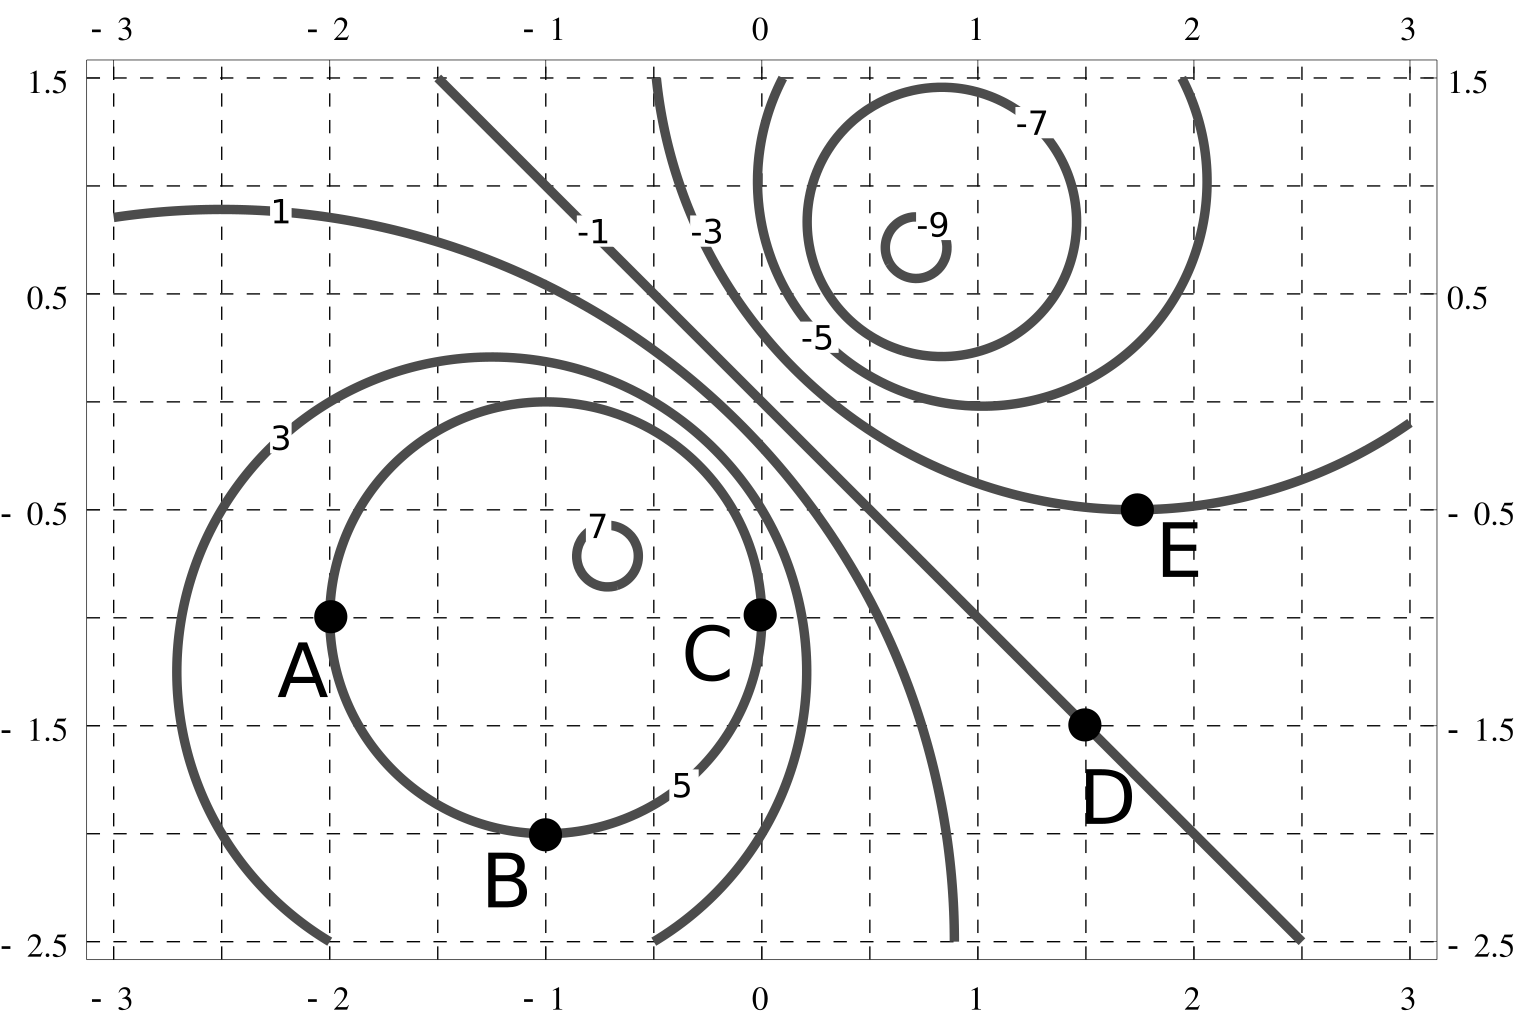
\includegraphics[width=4in]{contours1.png}
\end{image}
Assume $F(x,y)$ either strictly increases or decreases between contour lines.  List all points (\textsf{A}, \textsf{B}, \textsf{C}, \textsf{D},
\textsf{E}) where:

\begin{center}
\begin{tabular}{llll}
I. $\pp[F]{x}=0$.  \qquad \qquad &II. $\pp[F]{y}=0$. \qquad \qquad &III. $\pp[F]{x}>0$. \qquad \qquad &IV. $\pp[F]{y}<0$.
\end{tabular}
\end{center}

\begin{freeResponse}
Note that the contour plot shows the level curves of the function $F(x,y)$ in the $xy$-plane, and gives the value that the function takes along them.  For instance, the points $A$, $B$, and $C$ lie along the level curve associated to $z=5$.

An important observation is the following:

\begin{quote}
The tangent line to a level curve gives the direction in which the instantaneous rate of change of the function is $0$.
\end{quote}

I. $F_x(a,b)$ is the instantaneous rate of change of the function at $(a,b)$ in the $x$-direction.  Thus, to find the points at which $F_x=0$, we need to look for the locations where the tangent line to the level curve is in the $x$-direction.  This occurs at points $B$ and $E$.

II. $F_y(a,b)$ is the instantaneous rate of change of the function at $(a,b)$ in the $y$-direction.  Thus, to find the points at which $F_y=0$, we need to look for the locations where the tangent line to the level curve is in the $y$-direction.  This occurs at points $A$ and $C$.

III. To find where $F_x>0$, we need to look for when the function increases in the $x$-direction.  Since the function either must increase or must decrease between contours, note

\begin{itemize}
\item As $x$ increases from point $A$, we move from the contour curve along which $z=5$ to the one where $z=7$.  Thus, $F_x>0$ at $A$.
\item As $x$ increases from point $B$ or $C$, we move from the contour curve along which $z=5$ to the one where $z=3$.  Thus, $F_x<0$ at both $B$ and $C$.
\item The function must decrease between the contour curves along which $z=-1$ and $z=-3$, so $F_x<0$ at $D$.
\item We've said already that $F_x =0$ at $E$.
\end{itemize}

IV. To find where $F_y<0$, we need to look for when the function increases in the $x$-direction.  Since the function either must increase or must decrease between contours, note

\begin{itemize}
\item As $y$ increases from point $A$ or $C$, we move from the contour curve along which $z=5$ to the one where $z=3$.  However, the tangent lines to the level curve are in the $y$-direction at each of these points, so $F_y=0$ at each of these points.

\item As $y$ increases from point $B$, we move from the contour curve along which $z=5$ to the one where $z=7$.  Thus, $F_y>0$ at $B$.
\item As $y$ increases from point $D$, we move from the contour curve along which $z=-1$ to the one where $z=-3$.  Thus, $F_y<0$ at $D$.
\item As $y$ increases from point $E$, we move from the contour curve along which $z=-3$ to the one where $z=-5$.  Thus, $F_y<0$ at $E$.
\end{itemize}

%Add to gradient section!

\end{freeResponse}
\end{problem}

%%%%%%%%%%%%%%%%%%%%%%%%%%%%%%%%%%%%%%%%%%%%%%%%%

\begin{problem}
Let $f:\R^2 \to \R$ and let $z=f(x,y)$ be the surface associated to the function.

I. Classify the following as scalars, vectors in $\R^2$, or vectors in $\R^3$.

\begin{center}
\begin{tabular}{lll}
A. $f(1,2)$ \qquad \qquad \qquad & B. $\grad{f}(1,2)$  \qquad \qquad \qquad & C. $f_x(1,2)$ 
\end{tabular}
\end{center}

II. Classify the following as subsets of $\R$, $\R^2$, or $\R^3$.

\begin{center}
\begin{tabular}{ll}
A. The level curve through $(1,2)$. \qquad \qquad & B. The domain of $f(x,y)$. \\
C. The range of $f(x,y)$. & D. The surface $z=f(x,y)$. 
\end{tabular}
\end{center}

\begin{freeResponse}
I. $f(1,2)$ and $f_x(1,2)$ are scalars, $\grad{f}(1,2)$ is a vector in $\R^2$.

II. The level curve and the domain are subset of $\R^2$, the range is a subset of $\R$, and the actual surface $z=f(x,y)$ is a subset of $\R^3$.

\end{freeResponse}
\end{problem}

%%%%%%%%%%%%%%%%%%%%%%%%%%%%%%%%%%%%%%%%%%%%%%%%%

\section{Group Work}

\begin{problem}
Compute $\pderiv{f}{x}$ and $\pderiv{f}{y}$ for the following functions.  Then, write down $\grad{f}(x,y)$.
\begin{center}
\begin{tabular}{lll}
I. $f(x,y) = 2x+4xy^2$ \qquad & II. $f(x,y) = x \sin(x^2y)$ \qquad & III. $f(x,y) = \sqrt{5x+3\ln(2x+y)}$.
\end{tabular}
\end{center}

\begin{freeResponse}
To compute partial derivatives, treat the other variables as constants, and differentiating expressions involving the variable of differentiation exactly as before.  

To form the gradient, note that it is a vector whose $x$-component is the function $f_x(x,y)$ and its $y$-component is the function $f_y(x,y)$.
%%%%%%%
I. For $f(x,y) = 2x+4xy^2$, $f_x(x,y) = 2+4y^2$ and $f_y=8xy$.  Thus, 

\[
\grad{f}(x,y) = \vector{2+4y^2, 8xy}
\]
%%%%%%%
II. For $f(x,y) = x\sin(x^2y)$, notice the following.

\begin{itemize}
\item For $f_x(x,y)$, it is necessary to use the product rule, and we find that $f_x(x,y) = \sin(x^2y)+2x^2y \cos(x^2y)$.
\item For $f_y(x,y)$, it is not necessary to use the product rule since the first term in the product does not depend on $x$ explicitly.  Thus, $f_y(x,y) = \pp{y}\left[x \sin(x^2y)\right]= x\pp{y}\left[ \sin(x^2y)\right] = x^3\cos(x^2y)$.
\end{itemize}
 
\[
\grad{f}(x,y) = \vector{\sin(x^2y)+2x^2y \cos(x^2y), x^3\cos(x^2y)}
\]
%%%%%%%
III. For $f(x,y) = \sqrt{5x+3\ln(2x+y)}$, we have to differentiate carefully.

\begin{itemize}
\item For $f_x(x,y)$, we can compute

\begin{align*}
f_x(x,y) &= \frac{1}{2}\big( 5x+3\ln(2x+y) \big)^{-1/2} \cdot \pp{x} \bigg[ 5x+3\ln(2x+y)\bigg] \\
&= \frac{1}{2}\big( 5x+3\ln(2x+y) \big)^{-1/2} \cdot \left(5+\frac{6}{2x+y}\right) \\
&=\big( 5x+3\ln(2x+y) \big)^{-1/2} \cdot \left(\frac{5}{2}+\frac{3}{2x+y}\right) \\
\end{align*}

\item For $f_y(x,y)$, we can compute

\begin{align*}
f_y(x,y) &= \frac{1}{2}\big( 5x+3\ln(2x+y) \big)^{-1/2} \cdot \pp{y} \bigg[ 5x+3\ln(2x+y)\bigg] \\
&= \frac{1}{2}\big( 5x+3\ln(2x+y) \big)^{-1/2} \cdot \left(\frac{3}{2x+y}\right) \\
&= \big( 5x+3\ln(2x+y) \big)^{-1/2} \cdot \left(\frac{3}{4x+2y}\right) \\
\end{align*}
 
\end{itemize}

Writing out the gradient as before then factoring out the common term in the partials gives
\[
\grad{f}(x,y) =\big( 5x+3\ln(2x+y) \big)^{-1/2}\cdot \vector{ \frac{5}{2}+\frac{3}{2x+y}, \frac{3}{4x+2y}}.
\]

\end{freeResponse}
\end{problem}

%%%%%%%%%%%%%%%%%%%%%%%%%%%%%%%%%%%%%%%%%%%%%%%%%

\begin{problem}
Consider the function $f(x,y) = \frac{\cos(xy)}{x}$.

I. State the domain of the function.

II. Calculate both $f_{xy}(x,y)$ and $f_{yx}(x,y)$ in the order they are written.

III. Does Clairaut's Theorem hold for every $(x,y)$ in the domain?

\begin{freeResponse}
I. The domain of the function is $\left\{(x,y) \in \R^2 ~ \big| ~ x \neq 0\right\}$.

II. We first find the first order partial derivatives.

\begin{itemize}
\item For $\pp[f]{x}$, we use the quotient rule and find that 

\[
\pp[f]{x} = \frac{-xy\sin(xy)-\cos(xy)}{x^2} = -\frac{y}{x}\sin(xy)-\frac{1}{x^2}\cos(xy)
\]

\item For $\pp[f]{y}$, the quotient rule is not necessary since the denominator does not depend on $y$ explicitly. 

\[
\pp[f]{y} = \pp{y} \bigg[\frac{\cos(xy)}{x}\bigg] = \frac{1}{x} \cdot \pp{y} \bigg[\cos(xy)\bigg] = \frac{1}{x} \cdot \bigg[-x\sin(xy)\bigg] = -\sin(xy)
\]
\end{itemize}

Now we can compute the second order partial derivatives.

\begin{itemize}
\item Note that $f_{xy}(x,y) = \pp{y} \bigg[f_x\bigg]$, so

\begin{align*}
f_{xy}(x,y) &= \pp{y} \bigg[  -\frac{y}{x}\sin(xy)-\frac{1}{x^2}\cos(xy)  \bigg] \\
&=  \cancel{-\frac{1}{x}\sin(xy)}-y\cos(xy)+\cancel{\frac{1}{x}\sin(xy)}  \\
&=-y\cos(xy)
\end{align*}

\item Similarly, $f_{yx}(x,y) = \pp{x} \bigg[ f_y\bigg]$, so

\begin{align*}
f_{xy}(x,y) &= \pp{x} \bigg[ -\sin(xy)  \bigg] \\
&=  -y\cos(xy)
\end{align*}
\end{itemize}

III. The functions $f_{xy}(x,y)$ and $f_{yx}(x,y)$ are equal.  

\begin{remark}
Note that although $f_{xy}(x,y)$ and $f_{yx}(x,y)$ appear to be defined for all $(x,y)$, in performing many of the calculations, we need that $x \neq 0$.  This arose when we ``cancel'' the $x$ in the numerator and the denominator in the calculations for $f_y$, and clearly, $f_x$ is not even defined at $x=0$.  The domain of both $f_{xy}(x,y)$ and $f_{yx}(x,y)$ is thus $\left\{(x,y) \in \R^2 ~ \big| ~ x \neq 0\right\}$, which should not be too surprising in the sense that the partial derivatives certainly cannot be defined where the original function is not defined.

Since $f_{xy}(x,y)$ and $f_{yx}(x,y)$ are continuous where defined, Clairaut's Theorem tells us that they will be equal, which we explicitly saw by calculating them.
\end{remark}
\end{freeResponse}

\end{problem}

%%%%%%%%%%%%%%%%%%%%%%%%%%%%%%%%%%%%%%%%%%%%%%%%%

\begin{problem}
The \emph{heat equation} is a partial differential equation that describes how heat diffuses through a medium.  In the absence of a heat source, the equation is
\[
u_t(x,t) = k u_{xx}(x,t),
\]
where $k$ is the \emph{thermal diffusivity}, which measures the ability of a material to conduct thermal energy relative to its ability to store thermal energy.

If $k=2$, is $u(x,t) = e^{-4t}\cos(2x)$ a solution to the heat equation?  If not, what must $k$ be so the given function is a solution?

\begin{freeResponse}

We must determine if the function $u(x,t) = e^{-4t}\cos(2x)$ is a solution to $u_t(x,t) = 2 u_{xx}(x,t)$, which we can determine by computing the partial derivatives, substituting them into the partial differential equation (PDE), and checking whether the PDE is satisfied for all $(x,t)$.

\begin{itemize}
\item To compute $u_t$, note that 
\begin{align*}
u_t = \pp{t} \bigg[ e^{-4t}\cos(2x) \bigg] = \cos(2x) \cdot \pp{t} \bigg[ e^{-4t} \bigg] &= \cos(2x) \cdot \bigg[ -4e^{-4t} \bigg] \\
u_t &= -4e^{-4t}\cos(2x)
\end{align*}
\item Similarly,  $u_x = -2e^{-4t}\sin(2x)$, so $u_{xx} =-4e^{-4t}\cos(2x)$
\end{itemize}

Since $u_t(x,t) \neq 2 u_{xx}(x,t)$, $u(x,t) = e^{-4t}\cos(2x)$ is not a solution to $u_t(x,t) \neq 2 u_{xx}(x,t)$.

However, since we just found that $u_t(x,t) = u_{xx}(x,t)$, it is a solution to the equation $u_t(x,t) = k u_{xx}(x,t)$ when $k=1$.

\begin{remark}
In practice, to study the temperature evolution for a rod that extends from $x=0$ to $x=L$, we need both an initial temperature profile $u(x,0)$ (i.e. the initial temperature at each point) and boundary conditions at $x=0$ and $x=L$ that describe how the rod interacts with its external environment.  This type of problem is studied (and the above equation is derived) inmost classes in which one studies partial differential equations, like Math $2173$, $2177$, or $2415$.
\end{remark}

\end{freeResponse}


\end{problem}

%%%%%%%%%%%%%%%%%%%%%%%%%%%%%%%%%%%%%%%%%%%%%%%%%

%\begin{problem}
%Suppose that $f$ and $g$ are differentiable functions whose domain is $\R$ and let $c \in \R$.  
%
%I. Show that \[u(x,t) = \frac{1}{2} f(x-ct)+\frac{1}{2}f(x+ct)+\frac{1}{2c}\int_{x-ct}^{x+ct} g(s) \d s\] is a solution to the \emph{wave equation}
%
%\[
%\pderiv{^2u}{x^2} = \frac{1}{c^2} \pderiv{^2u}{t^2}.
%\]
%(This is called \emph{d'Alembert's solution} to the wave equation).
%
%II. What is $u(x,0)$?  What about $u_x(0,t)$?
%
%III.  Suppose that $f(s) = \cos(s)$ and $g(s) =2s$.  Explicitly construct the d'Alembert solution $u(x,t)$, then check explicitly that it satisfies the wave equation.
% 
%\begin{freeResponse}
%
%\end{freeResponse}
%
%%Move to homework; add gradient = 0 problem
%\end{problem}




\end{document}
